\documentclass[a4paper]{article}
\usepackage[T1]{fontenc}
\usepackage[utf8]{inputenc}
\usepackage{lmodern}
\usepackage{amsmath,amssymb}
\usepackage[top=3cm,bottom=2cm,left=2cm,right=2cm]{geometry}
\usepackage{fancyhdr}
\usepackage{esvect,esint}
\usepackage{xcolor}
\usepackage{tikz,circuitikz}\usetikzlibrary{calc}

\parskip1em\parindent0pt\let\ds\displaystyle

\begin{document}

\pagestyle{fancy}
\fancyhf{}
\setlength{\headheight}{15pt}
\fancyhead[L]{Electrocinétique}\fancyhead[R]{Question 29}

% Énoncé
\begin{center}
	\large{\boldmath{\textbf{Étude d’un passe-bas du deuxième ordre}}}
\end{center}

% Correction


On a $\underline{H}=\dfrac{1}{1+2\xi \dfrac{p}{\omega_0}+\dfrac{p^2}{\omega_0^2}},\quad p=j\omega,\quad\xi\in]0,1[$ \vspace{.2cm}\\
  $\omega\rightarrow 0 : \underline{H}\sim 1,\quad G=0\mathrm{dB},\quad \varphi=0$\\
  $\omega\rightarrow +\infty : \underline{H}\sim \dfrac{\omega_0^2}{p^2},\quad G=-40\log\omega+40\log\omega_0,\quad\varphi=-180^{\circ}$ \vspace{.3cm}\\

  $\underline{H}=\dfrac{1}{1+2j\xi \dfrac{\omega}{\omega_0}-\dfrac{\omega^2}{\omega_0^2}}$\hspace{1cm}
  $\underline{H}(\omega_0)=\dfrac{1}{2j\xi}\qquad\varphi(\omega_0)=-\dfrac{\pi}{2}=-90^{\circ}$\\
  $\varphi(\omega)=\arg \underline{H}=-\dfrac{\pi}{2}+\arctan \left( \dfrac{1- \dfrac{\omega}{\omega_0}}{2\xi \dfrac{\omega}{\omega_0}} \right)$\\
  $\varphi$ est décroissante de $0$ à $\pi$.

  \begin{center}
    \begin{tikzpicture}
      \draw [thick,->] (-2.5,0) to (2.5,0) node[anchor=north west]{\(\log\omega\)};
      \draw[thick,->](0,-2.5) to (0,2.5) node[anchor=south east]{\(\varphi\)};
      \draw (-2.5,0.1) to (0,0.1);
      \draw (0,-2) to (2.5,-2);
      \draw (0,-2) node [anchor= east ]{\(-180^{\circ}\)};
      \draw [red](-2.5,0.1) ..controls (0,0.1) and (0,-2)..(2.5,-2); 
      \draw (0,-1) node[anchor=north east]{\(-90^{\circ}\)};
    \end{tikzpicture}
  \end{center}

  $|\underline{H}|=\dfrac{1}{\sqrt{f(X)}}$ avec $X=\dfrac{\omega}{\omega_0}$\\
  $f(X)=(1-X^2)^2+4\xi^2X^2=1+X^4+(4\xi^2-2)X^2$\\
  $f'(X)=4X^3+4(2\xi^2-1)X=4X(X^2+2\xi^2-1)$


  \textbf{\(1^{\mathrm{ère}}\) étude :} amortissement fort $\xi>\dfrac{1}{\sqrt{2}}$\\
  
    $f'(X)$ a un seul zéro en $X=0$\\
  
  \begin{center}
    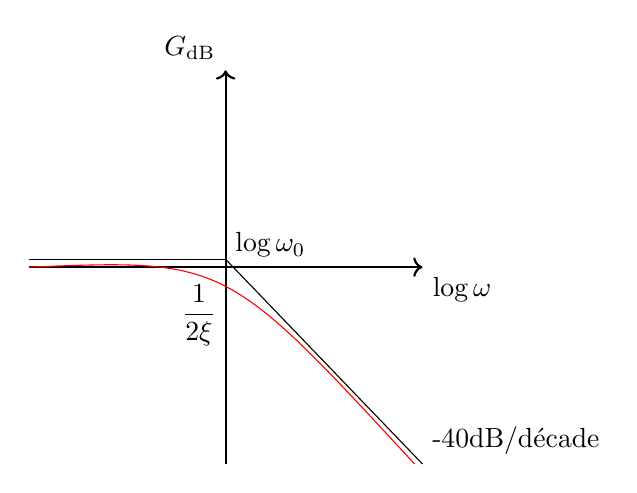
\begin{tikzpicture}
        \draw [thick,->] (-2.5,0) to (2.5,0) node[anchor=north west]{\(\log\omega\)};
        \draw[thick,->](0,-2.5) to (0,2.5) node[anchor=south east]{\(G_{\mathrm{dB}}\)};
        \draw (-2.5,0.1) to (0,0.1) ;
        \draw (0,0.1) to (2.5,-2.5) node[anchor=south west]{-40dB/décade};
        \draw (0,0) node[anchor=south west]{\(\log\omega_0\)};
        \draw [red](-2.5,0)..controls (0,0.1)..(2.4,-2.5);
        \draw (0,-0.1) node[anchor=north east] {\(\dfrac{1}{2\xi}\)};
    \end{tikzpicture}
  \end{center}


  \textbf{\(2^{\mathrm{ème}}\) étude :} amortissement faible $\xi<\dfrac{1}{\sqrt{2}}$\\
  
    $f'(X)$ a deux zéros en $X=0$ et en $X=\sqrt{1-2\xi^2}=X_0\\ (2\xi^2=1-X_0^2)$\\
    $f(X_0)=4\xi^2+4\xi^2(1-2\xi^2)=4\xi^2-4\xi^4=4\xi^2(1-\xi^2)$\\
    $\underline{H}(\omega_R)=\dfrac{1}{2\xi \sqrt{1-\xi^2}}$ avec $\omega_R=\omega_0 \sqrt{1-2\xi^2}$ pulsation de résonnance \vspace{0.15cm}\\
    Lorsque $\xi\rightarrow 0$, la résonnance devient infinie et la pulsation de résonnance tend vers la pulsation propre.
  
  \begin{center}
    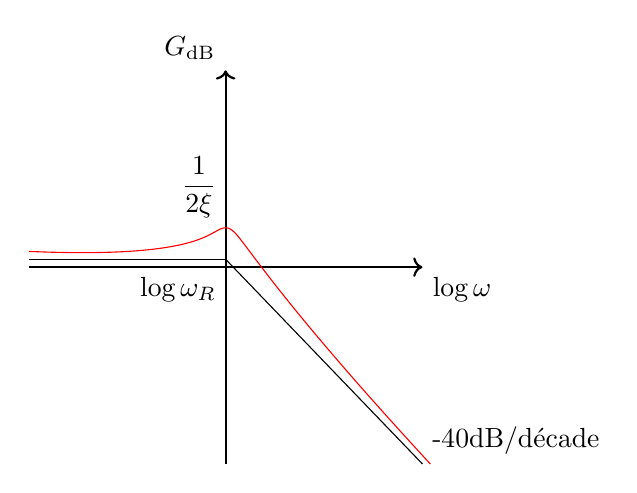
\begin{tikzpicture}
      \draw [thick,->] (-2.5,0) to (2.5,0) node[anchor=north west]{\(\log\omega\)};
        \draw[thick,->](0,-2.5) to (0,2.5) node[anchor=south east]{\(G_{\mathrm{dB}}\)};
        \draw (-2.5,0.1) to (0,0.1) ;
        \draw (0,0.1) to (2.5,-2.5) node[anchor=south west]{-40dB/décade};
        \draw (0,0) node[anchor=north east]{\(\log\omega_R\)};
        \draw [red] (-2.5,0.2) ..controls (-0.2,0.1) and (-0.2,0.5)..(0,0.5)..controls (0.2,0.5) and (0.2,0.1)..(2.6,-2.5);
        \draw (0,0.5) node[anchor=south east]{\(\dfrac{1}{2\xi}\)};
    \end{tikzpicture}
  \end{center}

\end{document}
